\section*{Appendix I: On Phase Singularities}

To construct the expression for an isolated optical vortex, we start from the wave equation
\begin{eqnarray}
	&&c^2\nabla^2\psi = \frac{\partial^2 \psi}{\partial t^2}.
	\label{eq:wave}
\end{eqnarray}
One can verify that wave functions of the form
\begin{eqnarray}
	&&\psi = (a + b\textcolor{blue}{y}) e^{i(kz - \omega t)}
	\label{eqn_301}
\end{eqnarray}
which are waves with linearly modulated amplitude, satisfy Eq. (\ref{eq:wave}). 
Now we consider two primary wave trains, say wave $A$ and $B$, assuming that they are monochromatic and modulated linearly along $y$-direction so that one rises, as the other falls. 
If wave $A$ and $B$ coincide with each other on the $y = 0$ plane with an angle $2 \alpha$ (see Fig. \ref{fig:two_primary_waves}), one can write down their wave expression
\begin{eqnarray}
	&&\psi_A = a_0(1 + \beta k_1 y) e^{i(k_1 x + k_3 z - \omega t - \pi/2)}
	\nonumber \\
	&&\psi_B = a_0(1 - \beta k_1 y) e^{i(-k_1 x + k_3 z - \omega t + \pi/2)}
	\label{eqn_302}
\end{eqnarray}
\textcolor{red}{Draw a schematic to represent $\psi_A$ and $\psi_B$.
	Resosolve the inconsistency between $\psi_A$, $\psi_B$ in (\ref{eqn_302}) and $\psi$ in (\ref{eqn_301}).}
where $\bar{k} = \hat{x} k_1 + \hat{z} k_3$ is the propagating vector of wave $A$, 
$a_0$ and $\beta$ are constants representing the amplitudes of carrier and modulating waves, respectively.

% Unable to show figure?
%\begin{figure}[h]
%	\vskip 6 cm
%	\hskip 0.3 cm
%	\special{wmf: primary_waves.pdf x=7 cm y=6 cm}
%	\caption{Illustration for the primary waves $A$ and $B$.}
%	\label{fig:two_primary_waves}
%\end{figure}
\begin{figure}[h]
	\centering
	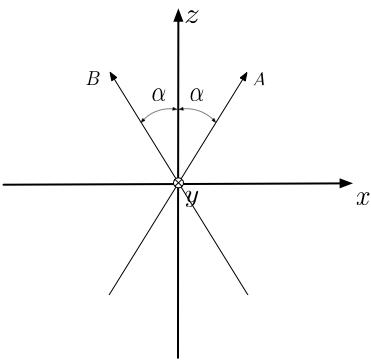
\includegraphics[width = 0.4\textwidth]{primary_waves.pdf}
	\caption{Illustration for the primary waves $A$ and $B$.}
	\label{fig:two_primary_waves}
\end{figure}

Let $c = \omega/k$, $k_1 = k \sin \alpha$, $k_3 = k \cos \alpha$, $\xi = k_1 x$, $\zeta = k_3 z - \omega t$ and $\eta = k_1 y$. 
The resultant complex wave field can be represented by the superposition of $A$ and $B$,
\begin{eqnarray}
	&&\psi = \psi_A + \psi_B = a_0 \left[ ( 1 + \beta \eta ) e^{i(\xi + \zeta - \pi/2)} \right. 
	\nonumber\\
	&&\hspace{0.3in} \left. + ( 1 - \beta \eta ) e^{i (- \xi + \zeta + \pi/2)} \right]
	\nonumber\\
	&&= 2 a_0 e^{i\zeta} \left[ \cos(\xi - \pi/2) + i \beta \eta \sin(\xi - \pi/2) \right]
	\nonumber\\
	&&= 2 a_0 e^{i\zeta} \left( \sin \xi - i \beta \eta \cos\xi \right)
	\nonumber
\end{eqnarray}
Therefore we can explicitly write down the formula of the wave in complex forms, \textcolor{blue}{$\psi = |\psi| e^{i\Phi}$,}
\textcolor{red}{What are $\rho$ and $\Phi$?}
\begin{eqnarray}
	&&\textcolor{blue}{|\psi|^2} = 4a_0^2 (\sin^2 \xi + \beta^2 \eta^2 \cos^2 \xi)
	\nonumber\\
	&&\Phi = 2n\pi + \zeta - \arctan\left(\frac{\beta \eta}{\tan \xi} \right).
\end{eqnarray}
Now, put $A_0 = 2a_0 \sin\alpha$ and let $\alpha \rightarrow 0$ without changing $A_0$ and $k$,
\begin{eqnarray}
	&&\textcolor{blue}{|\psi|^2} = A_0^2 \left[ \frac{\sin^2 (k\sin\alpha)x}{\sin\alpha^2} + \beta^2 k^2 y^2 \cos^2(k\sin\alpha)x \right]
	\nonumber\\
	&& \hspace{0.15in} \rightarrow A_0^2\left( k^2 x^2 + \beta^2 k^2 y^2 \right)
\end{eqnarray}
and
\begin{eqnarray}
	&&\Phi = 2n\pi + \left[(k \cos\alpha) z - \omega t \right] - \arctan\left(\frac{\beta \eta}{\tan \xi} \right)
	\nonumber\\
	&& \hspace{0.15in} \rightarrow 2n\pi + (kz - \omega t) - \arctan\left(\beta y/ x\right).
	\label{eq:limit}
\end{eqnarray}

Set $\beta = 1$ and represent Eq. (\ref{eq:limit}) in cylindrical coordinates, i.e. $(r, \phi, z)$ with $r^2 = x^2 + y^2, \phi = \arctan(y/x), z = z$,
\begin{eqnarray}
	\psi(r, \phi, z) = A_0 kr e^{i(k z - \omega t - \phi)}.
	\label{eq:single_vortex}
\end{eqnarray}
Eq. (\ref{eq:single_vortex}) characterizes an isolated skew-dislocation \cite{Ber73} of ``strength'' $m = 1$.

Having established the method to find the equation for a skew-dislocation by mixing two primary waves and performing a limiting process, Nye and Berry \cite{Ber73} claimed that these field expressions can be guessed \emph{a priori}. Therefore we need only generalize the present complex wave function $\psi$ we already have and keep they still satisfy the wave equation Eq. (\ref{eq:wave}). By this, we shall interpret the yielded functions as representing various kinds of dislocations, namely vortices.

In this perspective, Eq. (\ref{eq:single_vortex}) can be extended to the form
\begin{eqnarray}
	\psi = \left[ Ar^m + \left( \frac{B}{r^m} \right)\right] e^{i(kz - \omega t \pm m \phi)},
	\label{eq:vortex_m}
\end{eqnarray}
which still complies with Eq. (\ref{eq:wave}). Eq. (\ref{eq:vortex_m}) describes vortices with strength, or more precisely, topological charge, equals $m$. To define the topological charge, we consider a closed curve $C$ in the $(\bar{r}, t)$-space and perform the following steps:
\begin{enumerate}
	\item Around the curve $C$ the phase angle $\Phi$ may undergo a change of $2n \pi$, with $n \in \mathbb{Z}$ and $n \neq 0$.
	\item Shrink the closed curve $C$ to an arbitrarily small loop without changing $n$.
	\item If such a curve $C$ can be found, then $C$ is claimed to enclose a singularity because $\Phi$ varies infinitely fast 
	around the center point.
	\item The smoothness of the function $\psi$ implies that this scenario can only happen at points where $\psi = 0$, where $\Phi$ is not well-defined.
\end{enumerate}
A winding number $S_C$, characterizing the strength of this singularity, is defined as 
\begin{eqnarray}
	S_C = \frac{1}{2 \pi} \oint_C d \Phi = \frac{1}{2 \pi} \oint_C \nabla \Phi \cdot d \bar{r}
\end{eqnarray}
where $C$ is a contour enclosing the singularity.

\textcolor{blue}{
\section*{Appendix II: 2-D Fourier Transformation of Vortex Beam}
To compute the counterpart in frequency domain of the field $U(r, \phi, 0) = e^{i\phi}$, we recall the Fourier transformation pair
\begin{eqnarray}
A(f_x, f_y, z) = \int_{-\infty}^{\infty} \int_{-\infty}^{\infty} U(x, y, z)
e^{-i 2 \pi (f_x x + f_y y)} dx dy
\nonumber\\
U(x, y, z) = \int_{-\infty}^{\infty} \int_{-\infty}^{\infty} A(f_x, f_y, z)
e^{i 2 \pi (f_x x + f_y y)} df_x df_y.
\nonumber
\end{eqnarray}
Perform the following change of variable:
\begin{eqnarray}
	x = r\cos\phi & y = r\sin\phi & r \ge 0, 0 \le \phi \le 2\pi
	\nonumber\\
	f_x = \rho\cos\chi & f_y = \rho\sin\chi & \rho \ge 0, 0 \le \chi \le 2\pi
	\nonumber
\end{eqnarray}
Thus, we have
\begin{eqnarray}
	&&dx dy = r dr d\phi, \hspace{0.1in} df_x df_y = \rho d\rho d\chi,
	\nonumber\\
	&&xf_x + yf_y = r\rho \cos(\phi - \chi).
	\nonumber
\end{eqnarray}
To sum up, the 2-D Fourier transformation pair in cylindrical coordinate is represented by
\begin{eqnarray}
	A(\rho, \chi, z) = \int_{0}^{2\pi} \int_{0}^{\infty} U(r, \phi, z)
	e^{-i 2 \pi r \rho \cos(\phi - \chi)} r dr d\phi
	\nonumber\\
	U(r, \phi, z) = \int_{0}^{2\pi} \int_{0}^{\infty} A(\rho, \chi, z)
	e^{i 2 \pi r \rho \cos(\phi - \chi)} \rho d\rho d\chi.
	\nonumber
\end{eqnarray}
}

\textcolor{blue}{
Therefore, one can compute $\mathcal{F}\{e^{i\phi}\}$ as follows:
\begin{eqnarray}
	&&A(\rho, \chi, 0) = \int_{0}^{2\pi} e^{i\phi} 
		\left(\int_{0}^{\infty} e^{-i2\pi \rho r \cos(\phi - \chi)} r dr\right) d\phi
	\nonumber\\
	&&\hspace{0.5in}= \int_{0}^{2\pi} \frac{-e^{i\phi}}{4 \pi^2 \rho^2 \cos^2(\phi - \chi)} d\phi
	\nonumber\\
	&&\hspace{0.5in}= \frac{1}{\pi^2 \rho^2} \int_{0}^{2\pi} \frac{-e^{i\phi} d\phi}{e^{i(\phi - \chi)} + e^{-i(\phi - \chi)}}
	\nonumber\\
	&&\hspace{0.5in}= \frac{ e^{i\chi} }{\pi^2 \rho^2} \int_{\chi}^{\chi + 2\pi}
		\frac{-e^{i\phi'} d\phi'}{e^{i\phi'} + e^{-i\phi'}},
	\hspace{0.1in} (\phi' = \phi - \chi)
	\nonumber\\
	&&\hspace{0.5in}= \frac{i e^{i \chi}}{\pi^2 \rho^2} \oint_C \frac{dz}{(z + z^{-1})^2}
	\nonumber\\
	&&\hspace{0.5in}= \frac{i e^{i \chi}}{\pi^2 \rho^2} \oint_C \frac{z^2 dz}{(z^2 + 1)^2},
\end{eqnarray}
where the last complex contour integration is performed counterclockwise along the boundary $C$ of unit circle centered at the origin. Since the integrand in the last equality has two poles of order $2$ located at $i$ and $-i$ (both are on $C$), respectively, the contour integration can only be defined by Cauchy principal value, i.e.
\begin{eqnarray}
	{\cal P} \oint_C \frac{z^2 dz}{(z^2 + 1)^2} = \lim_{\epsilon \rightarrow 0} \oint_{C_{\epsilon}} \frac{z^2 dz}{(z^2 + 1)^2},
	\label{eq:CPV}
\end{eqnarray}
where $C_{\epsilon}$ is a curve defined as Fig. \ref{fig:contour}.
% Unable to show figure?
%\begin{figure}[h]
%	\vskip 6 cm
%	\hskip 0.3 cm
%	\special{wmf: contour.pdf x=7 cm y=6 cm}
%	\caption{Contour of $C_{\epsilon}$.}
%	\label{fig:contour}
%\end{figure}
\begin{figure}
	\centering
	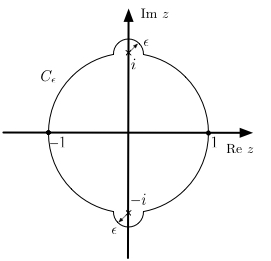
\includegraphics[width = .4\textwidth]{contour.pdf}
	\caption{Contour of $C_{\epsilon}$, which is formed by the boundary of the union of the unit circle centered at the origin and two circles with radius $\epsilon$ centered at $i, -i$, repectively.}
	\label{fig:contour}
\end{figure}
Note that $C_{\epsilon} \rightarrow C$ as $\epsilon \rightarrow 0$. The contour integration on $C_{\epsilon}$, on the other hand, can be evaluated by residue theorem.
\begin{eqnarray}
\oint_{C_{\epsilon}} \frac{z^2}{(z^2 + 1)^2} = 2\pi i \left( {\rm Res}(f; i) + {\rm Res}(f; -i) \right),
\label{eq:thm_residue}
\end{eqnarray}
with $f$ denoting the integrand in Eq. (\ref{eq:CPV}). By invoking the identity ${\rm Res}(f; a) = 1/(n-1)! \lim_{z \rightarrow a} d^n (z - a)^n f(z) /dz^n$ for a pole $a$ of order $n$, the residues can be computed:
\begin{eqnarray}
	{\rm Res}(f; i) = 1/8, & {\rm Res}(f; -i) = 3/8.
	\nonumber
\end{eqnarray}
Hence, Eq. (\ref{eq:thm_residue}) yields
\begin{eqnarray}
	A(\rho, \chi, 0) = \frac{- e^{i \chi}}{\pi \rho^2}. (?)
\end{eqnarray}
}

\textcolor{blue}{
\section*{Appendix III: Paraxial Wave Eqation}
Given a monochromatic electromagnetic field $\tilde{U}(x, y, z) \exp(-i \omega t) = U(x, y, z)\exp[i (kz - \omega t)]$, we have known that it satisfies the Helmholtz equation
\begin{eqnarray}
	\left(\nabla^2 + k^2\right) \tilde{U}(x, y, z) = 0.
	\label{eq:helmholtz}
\end{eqnarray}
If we compute
\begin{eqnarray}
	\frac{\partial^2}{\partial z^2} U(x, y, z)e^{ikz} = e^{ikz}
		\left( \frac{\partial^2 U}{\partial z^2} + 2ik \frac{\partial U}{\partial z} - k^2 U \right),
	\nonumber
\end{eqnarray}
Then Eq. (\ref{eq:helmholtz}) becomes
\begin{eqnarray}
	\left(\frac{\partial^2}{\partial x^2} + \frac{\partial^2}{\partial y^2} + \frac{\partial^2}{\partial z^2} + 2ik \frac{\partial}{\partial z} \right) U(x, y, z) = 0
	\label{eq:helmholtz_2}
\end{eqnarray}
One can further simplify the equation by performing {\em the paraxial approximation}:
\begin{eqnarray}
	\left| \frac{\partial^2 U}{\partial z^2} \right| \ll \left| 2k \frac{\partial U}{\partial z} \right|,
	\label{eq:paraxial}
\end{eqnarray}
which can be interpreted physically that the variation along $z$-axis is so small that all of the light must travel nearly paralle to the $z$-axis. Therefore, Eq. (\ref{eq:helmholtz_2}) is reduced to
\begin{eqnarray}
	\left(\nabla_{\perp}^2 + 2ik \frac{\partial}{\partial z} \right) U(x, y, z) = 0.
	\label{eq:pwe}
\end{eqnarray}
Usually, laser beams satisfy the paraxial approximation (\ref{eq:paraxial}) very well, whence it is convenient to model them by Eq. (\ref{eq:pwe}).
}
